\section{Literature Review}
\subsection{Wind Tunnel}
A wind tunnel is a large tube with air moving inside. This movement of air is usually done by powerful fans.
\begin{center}
	\begin{figure}[H]
		\centering
		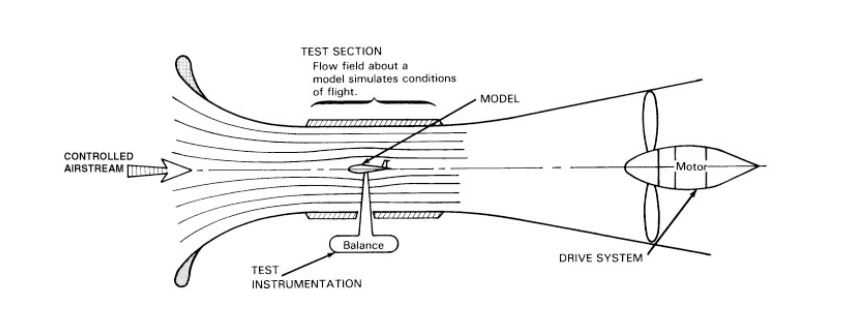
\includegraphics[width=0.7\linewidth]{Figures/Fig2}
		\caption[A Typical Wind Tunnel]{Diagram of a typical wind tunnel \cite{morris_force_2010}}
	\end{figure}
\end{center}
The first wind tunnel was built by Francis Wenham in 1871. However, it was the Wright Brothers who were the first to show the value of the wind tunnel in aerodynamic design with their 1902 wind tunnel. The Wright Brothers’ wind tunnel was largely made of wood, with a glass window on the top to look down through and see the force balance, from which the
lift and drag forces could be read. The wind tunnel was powered by a fan driven off a natural gas fuelled engine. Their tunnel was square of 16" by 16"(about 407mm by 407mm), and 6 foot long (about 1829mm), with a maximum test speed of 35 mph (about 56 km/h)\cite{morris_force_2010}.


Later in the early 20th century in Europe, the main users of wind tunnels were Gustave Eiffel in France and Ludwig Prandtl in Germany. Prandtl built the first closed circuit wind tunnel in 1908. Closed circuit wind tunnels are characterized by the recirculation of the airflow with very minimal exchange with the exterior. Open circuit wind tunnels on the other hand, have an airflow that follows a straight path and flows to the contracted zone where the test section is located and then passes through a diffuser, a fan section and an exhaust.

By the 1940’s supersonic wind tunnels were in use. In 1972, a cryogenic wind tunnel was built at NASA Langley by injecting liquid nitrogen into the wind tunnel to cool the gas. This lowered the viscosity and increased the Reynolds number, and this tunnel had the capability to match Reynolds and Mach numbers simultaneously up to Mach 1.2
\cite{fernandes_design_nodate}.

Today the largest wind tunnel in the world is the National Full-Scale Aerodynamics Complex at NASA's Ames Research Center, which has a test section of cross-section 80 ft by 100 ft (24 m x 31 m). The types of instruments in common use in wind tunnels include boundary layer rakes, tufts, pitot tubes, pressure sensitive paint, smoke, and static pressure taps \cite{morris_force_2010}.

NASA uses wind tunnels to test scale models of aircraft and spacecraft. The wind tunnels help to test ideas of making aeroplanes better and safer. They are also used to help engineers in designing spacecraft that will work in other planets such as mars - the wind tunnel can be used to simulate objects in an atmosphere that's thinner than ours e.g. an atmosphere that's exactly like the Martian atmosphere.
\begin{center}
	%&\vspace*{-4.0cm}
	\begin{figure}[H]
		\centering
		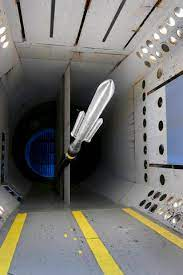
\includegraphics{Figures/Fig4}
		\caption[NASA Wind tunnel - space application]{NASA wind tunnels used to test the design of heavy-lift rocket \cite{NASA}}
	\end{figure}
\end{center}
NASA has wind tunnels of different types and sizes. Some are low-speed wind tunnels, others are hypersonic i.e. they are made to carry out tests at 4,000 mph (6437 kph) \cite{NASA}.
\subsection{Stewart Platform}
The Stewart platform is an example of a parallel manipulator.
Parallel link manipulators have become an important area of research due to their: precision, rigidity and high-load-to-weight ratio.
These manipulators find practical applications in flight simulators, precise machining and applications that require disturbance isolation \cite{iqbal_dynamic_2008}.

A Stewart platform is a parallel manipulator that provides six-degree-of-freedom (DOF) i.e. roll, pitch, yaw, surge, sway and heave (displacement in the z-direction), and can be controlled in all these freedoms simultaneously.
The platform consists six legs connecting a top plate to a base plate with spherical joints as the connection points.

The platform is able to move in three angular directions and in three linear directions, singly or in any combination \cite{stewart1965platform}. Angular and translational motion of the top plate with
respect to the base plate is achieved by reducing or extending the actuator lengths (for Stewart platforms with linear actuators for legs) or by writing various servo angles to the servo motors
(for Stewart platforms that use servo motors to actuate leg movements) \cite{iqbal_dynamic_2008}.

\subsubsection{Stewart Platform Configurations}
Stewart platforms can take three primary configurations i.e. 3-3 type, 3-6 type or 6-6 type.
\begin{center}
	\begin{figure}[H]
		\centering
		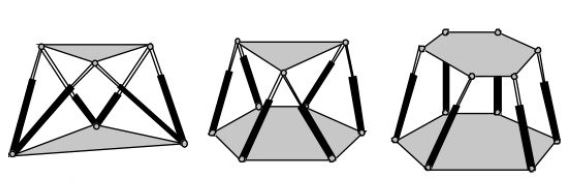
\includegraphics{Figures/stewart}
		\caption[Configurations]{Type 3-3, 3-6 and 6-6 respectively
			\cite{fernandes_design_nodate}}
	\end{figure}
\end{center}
The base and the platform (for the 3-3 type), and the platform (for the 3-6 type) are triangular in shape. The triangular shape has a good load carrying capability only in theory and for certain dimensions. These configurations are, however,not possible in practice since double spherical joints will be needed where two bars have to be joined at the same vertex
\cite{fernandes_design_nodate}.

For a 6-6 type Stewart platform, the base and platform are hexagon in shape.

\subsubsection{Inverse Kinematics of a Stewart Platform}
This is the calculation of each leg length based on the desired position of the Stewart platform.
For the Stewart platform, the translation $^{p}T_{b}$ from the base origin to the platform origin can be described with a single vector T = $(t_{x} t_{y} t_{z})^{T} $. The rotation of the platform can be denoted as $^{p}R_{b}$. Thus the following relationship for the frame of reference can be stated \cite{Eisele_2019}:
\begin{ceqn}
	\begin{align}
		^{p}T_{b} = T
	\end{align}
\end{ceqn}
\begin{ceqn}
	\begin{align}
		^{p}R_{b} = R
	\end{align}
\end{ceqn}
\begin{ceqn}
	\begin{align}
		^{b}T_{p} =(^{p}T_{b})^{-1} =T^{-1}
	\end{align}
\end{ceqn}
\begin{ceqn}
	\begin{align}
		^{b}R_{p} = (^{p}R_{b})^{-1}
	\end{align}
\end{ceqn}
\begin{center}
	\begin{figure}[!h]
		\centering
		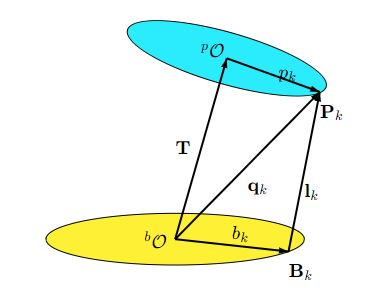
\includegraphics[width=0.4\linewidth]{Figures/servo2}
		\caption[Leg length]{Leg Length \cite{Eisele_2019}}
	\end{figure}
\end{center}
The leg length $l_{k}$ can therefore be found with:
\begin{ceqn}
	\begin{align}
		l_{k} = P_{k} - B_{k} = T + R \times p \times R^{-1} - b_{k}
	\end{align}
\end{ceqn}
Where,\\
$P_{k}$ - leg attachment on platform \\
$B_{k}$- leg attachment on base
\subsubsection{Inverse Kinematics Using Rotational Servo Motors}
For a rod of fixed length d between servo horn anchor $H_{k}$ and platform anchor $P_{k}$,  $H_{k}$ has a distance h between the original base anchor and servo shaft $B_{k}$. The vector h is perpendicular to the servo shaft and is rotated by angle $\alpha_{k}$ when lifted from the horizontal line.
\begin{center}
	\begin{figure}[!h]
		\centering
		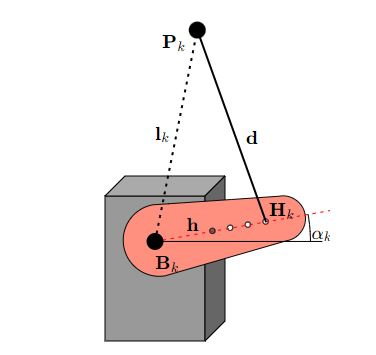
\includegraphics[width=0.4\linewidth]{Figures/servo}
		\caption[Servo angle]{Servo angle \cite{Eisele_2019}}
	\end{figure}
\end{center}
Derivation relationships of inverse kinematics are used to calculate each servo angle and is given as \cite{Eisele_2019}:
\begin{ceqn}
	\begin{align}
		\alpha_{k} = sin^{-1}(\frac{g_{k}}{\sqrt{e_{k}^2+f_{k}^2}})-arctan2(f_{k}, e_{k})
	\end{align}
\end{ceqn}
Where,
$$e_{k} = 2hl_{k}^{(z)} $$
$$e_{k} = 2h(cos(\beta_{k})I_{k}^{(x)}+sin({\beta_{k}})I_{k}^(y))$$
$$g_{k} = l_{k}^2 - (d^2 - h^2)   $$

\subsubsection{Quality Index ($\lambda$) of the Stewart Platform}
Quality index $(\lambda)$ varies from 0 to 1.\\
Where,\\
0 - design with singularities and\\
1 - Optimal design in which the determinant of the correspondent Jacobian matrix is maximum.

\textbf{Singularities} - uncontrollable states.

The Jacobian matrix relates the axial forces in the $i^{th}$ bar with the applied
forces and torques and is given in equation \eqref{eq:myeqn1} \cite{fernandes_design_nodate}:

\begin{ceqn}
	\begin{align}
		J =
		\begin{pmatrix}
			\hat{\boldsymbol{S_{1}}} & \hat{\boldsymbol{S_{2}}} & \hat{\boldsymbol{S_{3}}} & ... & \hat{\boldsymbol{S_{n}}}
		\end{pmatrix}
		\label{eq:myeqn1}
	\end{align}
\end{ceqn}

Where n - number of bars and $ \hat{\boldsymbol{S_{i}}}$ - unit vector of the Plucker coordinates along the line of the
$i_{th}$ bar.

Quality index can be obtained as shown:
\begin{ceqn}
	\begin{align}
		\lambda = \frac{|J|}{|J|_{m}}
		\label{eq:myeqn}
	\end{align}
\end{ceqn}
Where, $|J|$ is the determinant of the Jacobian matrix of a given Stewart platform configuration, and $ |J|_{m} $ - determinant of Jacobian Matrix of the optimal configuration.

Applying equation \eqref{eq:myeqn1} to the general configuration of a 6-6 platform, it is
possible to obtain the Jacobian matrix and thus its determinant which can be obtained as follows:
\begin{ceqn}
	\begin{align}
		|J| =
		\frac{81 \sqrt{3} a^3 b^3 h^3 (3 \alpha \beta - 2 \alpha - 2 \beta +1)^3}{4(a^2(3 \alpha^2 - 3 \alpha + 1)+ ab(\alpha \beta - 1 )+ b^2(3 \beta^2 - 3 \beta + 1)+ 3h^2)^3}
		\label{eq:myeqn02}
	\end{align}
\end{ceqn}
Where:\\
a - diameter of moving platform\\
b - diameter of base\\
$\alpha$ - angle of attack\\
$ \beta $ - Side slip angle\\
h - distance between the base and the moving platform\\

$|J|_{m}$ is found by differentiating equation \eqref{eq:myeqn02} with respect to h and equating to 0 resulting in \cite{fernandes_design_nodate}:
\begin{ceqn}
	\begin{align}
		h = \sqrt{\frac{1}{3}(a^2 (3 \alpha^2 - 3 \alpha + 1)+ ab (3\alpha\beta - 1)+b^2(3 \beta^2 - 3 \beta + 1))}
		\label{eq:myeqn3}
	\end{align}
\end{ceqn}

\subsection{Force Balances}
For wind tunnel applications, the wind axes is used as the reference frame. Where, X axis points to the accelerated air; Z axis points downward and; Y axis points to the right in the direction of the wind. In the reference frame above, lift is in the negative z-direction, drag in the negative x-direction and, side force in the negative y-direction \cite{bueno2018design}.

Moment components on the x,y,z axes are rolling moment, pitching moment and yawing moment respectively. A three-component force balance can be considered to measure the lift, drag and pitch (angle of attack).

Force balances can be external or internal. In external force balances the test section lies outside of the wind tunnel test section, whereas in internal force balances the balance is inside the model itself connecting the model to the support structure.
\subsubsection{External Force Balances}
Several different types of external force balances are available for wind tunnel use
\cite{morris_force_2010}:
\begin{enumerate}
	\item Wire
	\item Platform
	\item Yoke
	\item Pyramidal
\end{enumerate}
In the wire balance, the model under testing is suspended by wires each connected to an extensometer (a sensor that produces an electrical output when submitted to a load and deforms). The shortcoming of the wire balance is the large tare drag caused by the wires which is difficult to quantify. They are also not robust nor versatile enough compared with the other alternatives \cite{ferreira2015design}.
\begin{center}
	\begin{figure}[H]
		\centering
		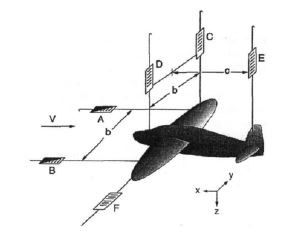
\includegraphics{Figures/Wire}
		\caption[Wire force balance]{Wire force balance \cite{ferreira2015design}}
	\end{figure}
\end{center}
The platform balance is relatively easy to construct, assemble and instrument. However, for this balance, forces and torques are coupled and the balance resolving center does not coincide with the center of the tunnel.
\begin{center}
	\begin{figure}[H]
		\centering
		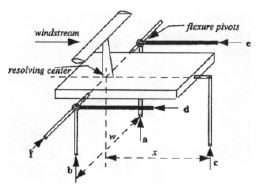
\includegraphics{Figures/platform}
		\caption[Platform force balance]{Platform force balance \cite{ferreira2015design}}
	\end{figure}
\end{center}
In the yoke balance configuration, forces and torques are coupled and the balance resolving center coincides with the center of the tunnel. This configuration, however, presents some structural deflections due to the large span of the measuring and support arms.
\begin{center}
	\begin{figure}[H]
		\centering
		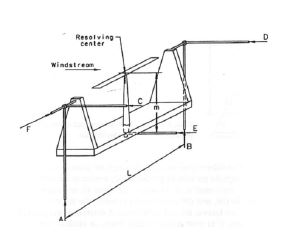
\includegraphics{Figures/Yoke}
		\caption[Yoke force balance]{Yoke force balance \cite{ferreira2015design}}
	\end{figure}
\end{center}
The pyramidal balance configuration is a further improvement of the yoke balance in order to overcome the shortcomings of the other balances. It is capable of measuring six components of forces and
torques separately and without coupling, provided that the balance is well assembled and calibrated.
\begin{center}
	\begin{figure}[H]
		\centering
		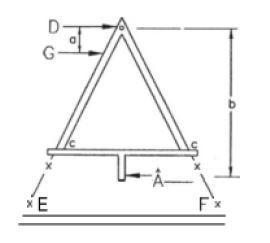
\includegraphics{Figures/Pyramid}
		\caption[Pyramid force balance]{Pyramid force balance \cite{ferreira2015design}}
	\end{figure}
\end{center}
It is possible to merge some of the force balance concepts to come up with an innovative, easy-to-manufacture and cost-effective external force balance. One such solution can be the use of a Stewart platform as a force balance. The Stewart platform offers another advantage - dynamic positioning of the model in the test section.
The platform bars are subjected to axial forces only and can have strain-gages coupled to each one as Wheatstone bridges. Forces and torques are then obtained based on the axial displacements obtained by the strain gages\cite{fernandes_design_nodate}.

Table \ref{tablecom} shows a summary of advantages and disadvantages of external force balances.
\clearpage
\begin{center}
	\begin{table}[H]
		\caption[Comparison of Force Balances]{A Table of Comparison and Contrast of External Force Balances}
		\label{tablecom}
	\end{table}
	\begin{tabular}{|l|l|l|}
		\hline
		\textbf{Type} & \textbf{Advantages}                         & \textbf{Disadvantages}        \\
		\hline
		Wire          & Relatively simple construction              & large tare drag               \\
		              &                                             & Less Versatile and robust     \\
		\hline
		Platform      & Easy construction and instrumentation        & Force and torques coupled     \\
		              &                                             & Center alignment difficulties \\
		\hline
		Yoke          & Overcomes center alignment problems         & Structural deflections        \\
		\hline
		Pyramidal     & Overcomes shortcoming of other balances     &                               \\
		              & Measures 6 components of forces and torques &                               \\
		\hline
	\end{tabular}
\end{center}
\subsubsection{Internal Force Balances}
The different kinds of internal balances can be made based on \cite{ferreira2015design}:
\begin{enumerate}
	\item The type of transducer i.e. strain gauge or piezoelectric balance.
	\item Shape i.e. box balance and sting balance
\end{enumerate}
\begin{center}
	\begin{figure}[H]
		\centering
		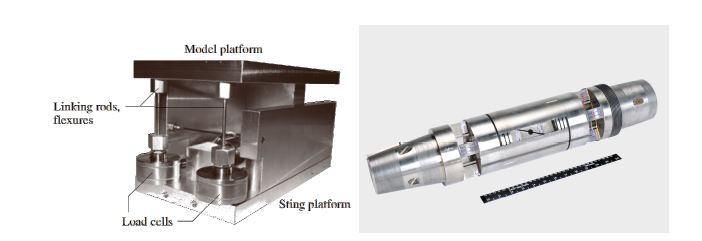
\includegraphics[width=0.8\linewidth]{Figures/Fig7}
		\caption[Internal force balances]{Typical configurations for internal force balances. \textit{Left to right:} Box balance and sting balance \cite{ferreira2015design}.}
	\end{figure}
\end{center}
The box balance presents a cubic shape and can either be made of a solid piece of material or from assembled parts. In this configuration, the loads are transferred from the top to the bottom. The sting balance presents a cylindrical shape and the loads are transferred from one end to the other in the longitudinal direction. It can be used to measure forces or torques.

The advantage of internal force balances is that they minimize the interference caused by the supporting bars in the flow.
\subsection{Sensors}
\subsubsection{Load Sensors}
Several methods can be used to measure forces and torques in a force balance. These methods can be generally grouped into two\cite{ferreira2015design}:
\begin{enumerate}
	\item Hydraulic measuring techniques.
	\item Electric measurement techniques.
\end{enumerate}
Electric measurement techniques are preferred for Force balance applications. One such electric measurement device is the strain gauge. A strain gauge is an electromechanical device whose electrical resistance changes linearly with the strain in the component.

Metal foil strain gauges are widely used. This type of strain gauges provide more precise strain values than wire strain gauges. However, since the relative changes on electric resistance of the strain gauge are so small, it is necessary to develop an effective method of measuring them because each strain gauge would require extremely accurate signal measurements. The solution is to have a set of strain gauges coupled in order to minimize the required accuracy, forming a force transducer i.e. the \textit{Wheatstone bridge}.
\begin{center}
	\begin{figure}[H]
		\centering
		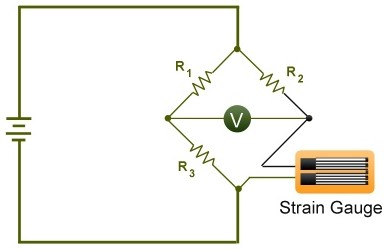
\includegraphics[width=0.6\linewidth]{Figures/Fig9}
		\caption[Wheatstone Bridge Circuit]{Wheatstone Bridge Circuit \cite{ferreira2015design}}
	\end{figure}
\end{center}
Load cells can also be used to measure the drag and lift forces\cite{ferreira2015design}.
\subsubsection{Attitude Sensor}
It is important to define the desired aerodynamic angles and to guarantee that they are measured accurately in relation to the air stream. One such angle is the angle of attack (\textalpha) shown in Figure \ref{att}. For this reason, specific devices that provide the attitude measurement should be implemented in order to improve the precision of the results.

Angle of attack (\textalpha)is the angle measured between the longitudinal axis of the model and the direction of the flow on a vertical (Figure \ref{att})
\begin{center}
	\begin{figure}[H]
		\centering
		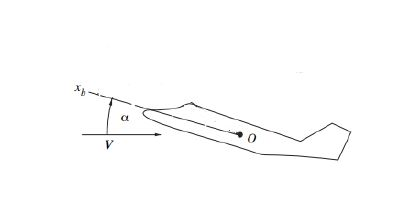
\includegraphics[width=0.6\linewidth]{Figures/Fig10}
		\caption[Angle of attack]{Angle of attack (\textalpha) \cite{ferreira2015design}}
		\label{att}
	\end{figure}
\end{center}

\subsection{Smoke visualization System for Wind Tunnel}
The ability to visualise the airflow over solid objects in a wind tunnel crucial in understanding the fundamental principles of both fluid dynamics and aerodynamics. To achieve this a uniform row of smoke lines are required. These smoke lines should be sufficiently long to maintain their integrity throughout
the test section \cite{trinder2013development}.

Smoke visualization methods including smoke-generating materials and techniques for generating smoke lines have been summarized in the tables below.
\begin{center}
	\begin{table}[H]
		\caption[Smoke Generating Materials]{Comparison of Smoke Generating Materials}
	\end{table}
	\begin{tabular}{|p{5cm}|p{5cm}|p{5cm}|}
		\hline
		\textbf{Material}                            & \textbf{Advantages}                 & \textbf{Disadvantages}                                      \\
		\hline
		Tobacco, kerosene and titanium-tetrachloride & Produces high quality smoke         & Hazardous/toxic; tobbacco is difficult to control           \\
		\hline
		Carbon dioxide                               & Produces dense smoke                & Potentially harmful in large volumes; needs to be exhausted \\
		\hline
		Water-based liquids                          & Non-hazardous; produce dense vapour & Vapour can condense back to liquid                          \\
		\hline
	\end{tabular}
\end{center}

\begin{center}
	\begin{table}[H]
		\caption[Smoke Generating Techniques]{Comparison of Smoke Generating Techniques}
	\end{table}
	\begin{tabular}{|p{5cm}|p{5cm}|p{5cm}|}
		\hline
		\textbf{Technique} & \textbf{Advantages}                                & \textbf{Disadvantages}                      \\
		\hline
		Smoke wire         & Produces the most effective smoke lines            & Complex set-up to achieve resistive heating \\
		\hline
		Smoke rake         & Can be utilised with non-hazardous smoke materials & Prone to wind tunnel blockage effects       \\
		\hline
	\end{tabular}
\end{center}
For smoke rake, an aerodynamically shaped
body (typically elliptical) featuring a row of tubes through which the smoke exits is used. Smoke to the rake can be introduced from a non-hazardous source,
such as a water-based liquid heated by a
smoke machine, rather than using combustion of hydrocarbons as in the smoke wire technique, which is hazardous and produces toxic materials \cite{trinder2013development}.

\subsection{Previous Work}
Force balance design for educational wind tunnels is an area of great interest. This is especially important
for aerodynamics studies of aeroplanes and aerofoil models, as well as ground vehicles such as trucks
and cars \cite{morris_force_2010}.

Force balances can be used in conjunction with a linear actuator where the
actuator is mounted inside the force balance apparatus, using a parallel four-bar linkage so that
the angle of attack is linearly related to the actuator position. Alternatively, manipulators such as the Stewart platform can serve as force balances. This section presents some of the work that has been done in this area.
\subsubsection{Bradley University (USA)}
The Mechanical Engineering department of Bradley University has a force balance installed in the test-section of a subsonic wind tunnel. The force balance comprises of two load cells to measure lift and drag forces. A linear actuator is used in conjunction with the force balance to change the angle of attack of models during testing.
\begin{center}
	\begin{figure}[H]
		\centering
		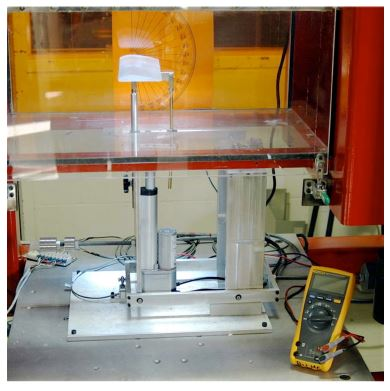
\includegraphics[width=0.6\linewidth]{Figures/force}
		\caption[Force balance installed]{Force balance installed in the wind tunnel \cite{morris_force_2010}}
	\end{figure}
\end{center}
There is a possibility of adding a third load cell to this configuration to enable measurement of the pitching moment. The force balance offers good results with lift and drag coefficients not changing by more than 10 percent with varying wind tunnel velocity in the range of Reynolds
numbers where the coefficients should be fairly constant \cite{morris_force_2010}.

The overall cost of coming up with this force balance is given as 1000 dollars which is significantly cheaper than the commercially available force balances. A two-component force balance goes for a minimum of 9385 dollars.
%\subsection{Inertial Measurement Units (IMUs)}
%IMU’s are sensors that combine an accelerometer, a gyroscope and, in other cases, a magnetometer.
%They're used widely due to their small size and low cost. The gyroscope measures the
%sensor’s angular velocity and the accelerometer is used to measure the external force acting on the
%sensor which is not only due to its acceleration but also to the gravity. The gyroscope measurements
%can provide the change in pitch, roll and yaw by integrating the values of angular velocities along the
%three axis, but to calculate absolute values of these angles, reference data is needed. This data can be
%obtained from the accelerometer or the magnetometer. It is possible to obtain pitch and roll angles from
%the accelerometer, putting  gravitational acceleration in consideration. However, yaw angle cannot
%be obtained directly from the results of the accelerometer as it is in the same direction as the gravity.
%For calculating yaw, the data from the magnetometer as reference and then integrates the gyroscope
%information \cite{ferreira2015design}.
%\begin{center}
%	\begin{figure}[H]
%\centering
%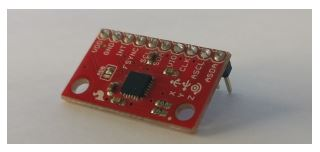
\includegraphics[width=0.6\linewidth]{Figures/imu}
%\caption[Inertial Measurement Unit]{IMU (MPU 6050) \cite{ferreira2015design}}
%\end{figure}
%\end{center}
\subsubsection{East Africa School of Aviation (EASA)}
The EASA Aerodynamics lab has a subsonic wind tunnel 300mm (AF1300) and a flight demonstration wind tunnel(AF41) supplied by TECQUIPMENT. The Subsonic wind tunnel is equipped with a three-component force balance, smoke generator, multi-tube manometer and a range of aerofoil drag, boundary layer low and high wing models. The Flight demonstration wind tunnel has a data acquisition module for classroom demonstrations and investigations into the behavior of fixed-wing aircraft and wing-performance during take-off, flight and landing \cite{TEC}.

\subsubsection{Tecnico Lisboa}
In 2018, Joao Fernandes of Tecnico Lisboa developed a force balance system to
be used with the aerospace engineering laboratory wind tunnel. The project was to
design a force balance measuring the six components. A Stewart platform was used as the
force and measurement system which was made possible through instrumentation of the platform legs.
For sensing, strain gauges were used and connected in a Wheatstone bridge configuration.
The system was able to measure all the six components of aerodynamic properties\cite{ferreira2015design}.

Further developments were made two years later to this design which are enumerated below \cite{ferreira2015design}:
\begin{enumerate}
	\item The use of a half bridge configuration of strain gauge for the measurement system.
	\item Use of an Arduino DAQ system for temperature and humidity monitoring to help in
	      compensation of switching to a half bridge configuration for the strain gauges.
\end{enumerate}
\subsubsection{Stewart Platform at JKUAT}
Six-DOF Stewart platforms have been designed and fabricated by students in the Mechatronic Engineering department as part of their final year projects. The Stewart platforms by the first two groups of students were for different applications and the one from FYP-17 was to be used as a force balance for Wind tunnel testing \cite{caleb}. Although the Stewart platform was built successfully, the group didn't achieve a force balance for the same.
\subsection{Summary of Gaps}
Whereas the Force balance by the Mechanical Engineering department in Bradley University is relatively simple to construct, it still poses a challenge in terms of cost. Cost can be minimized based on load cell and actuator selection but this does not guarantee that the level of accuracy will not be compromised. Also, only two or three force components can be obtained. The force balance setup doesn't allow dynamic positioning of models in the wind tunnel during testing.

Institutions such as EASA have procured their force balances. The force balances guarantee high accuracy but this may not be a cost-effective solution.

With so much research in the area of Stewart platform, there remains still more work to be done in the areas of control, dynamics, and singular positions.The Stewart platform force balance by Joao,for example, doesn't have actuation \cite{ferreira2015design}.

A 6 DOF Stewart platform with force measurement for a low-speed wind tunnel has been done as final year project in JKUAT under the department of Mechatronic Engineering (FYP 17). Whereas the former team was able to successfully design and assemble the platform, as well as the actuation circuitry, there still remains work to do in the following areas \cite{caleb}:
\begin{enumerate}
	\item Development of a Human-Machine-Interface for Stewart platform control.
	\item Data acquisition from sensors.
	\item Implementation of servo circuit control.
	\item Calibration of the measurement system to be in-line with NASA aerofoils.
\end{enumerate}